\documentclass{article}
\usepackage{float}
\usepackage{graphicx}
\usepackage{amsmath}
\usepackage{listings}
\usepackage{color}
\usepackage{multicol}
\usepackage{cancel}
\definecolor{cadmiumgreen}{rgb}{0.0, 0.42, 0.24}
\lstset{frame=tb,
  language=R,
  aboveskip=3mm,
  belowskip=3mm,
  showstringspaces=false,
  columns=flexible,
  basicstyle={\small\ttfamily},
  numbers=none,
  numberstyle=\tiny\color{gray},
  keywordstyle=\color{blue},
  commentstyle=\color{dkgreen},
  stringstyle=\color{cadmiumgreen},
  breaklines=true,
  breakatwhitespace=true,
  tabsize=3
}
\usepackage[margin=0.75in]{geometry}
\setlength\parindent{0pt}

\title{Seismo 512 HW 6}
\date{2/17/2023}
\author{Simon-Hans Edasi}

\begin{document}

	\maketitle

%%%%%%%%%%%%%%%%%%%%%%%%%%%%%%%%%%%%%%%%%%%%%%%%%%
\section{}

\begin{figure}[H]
    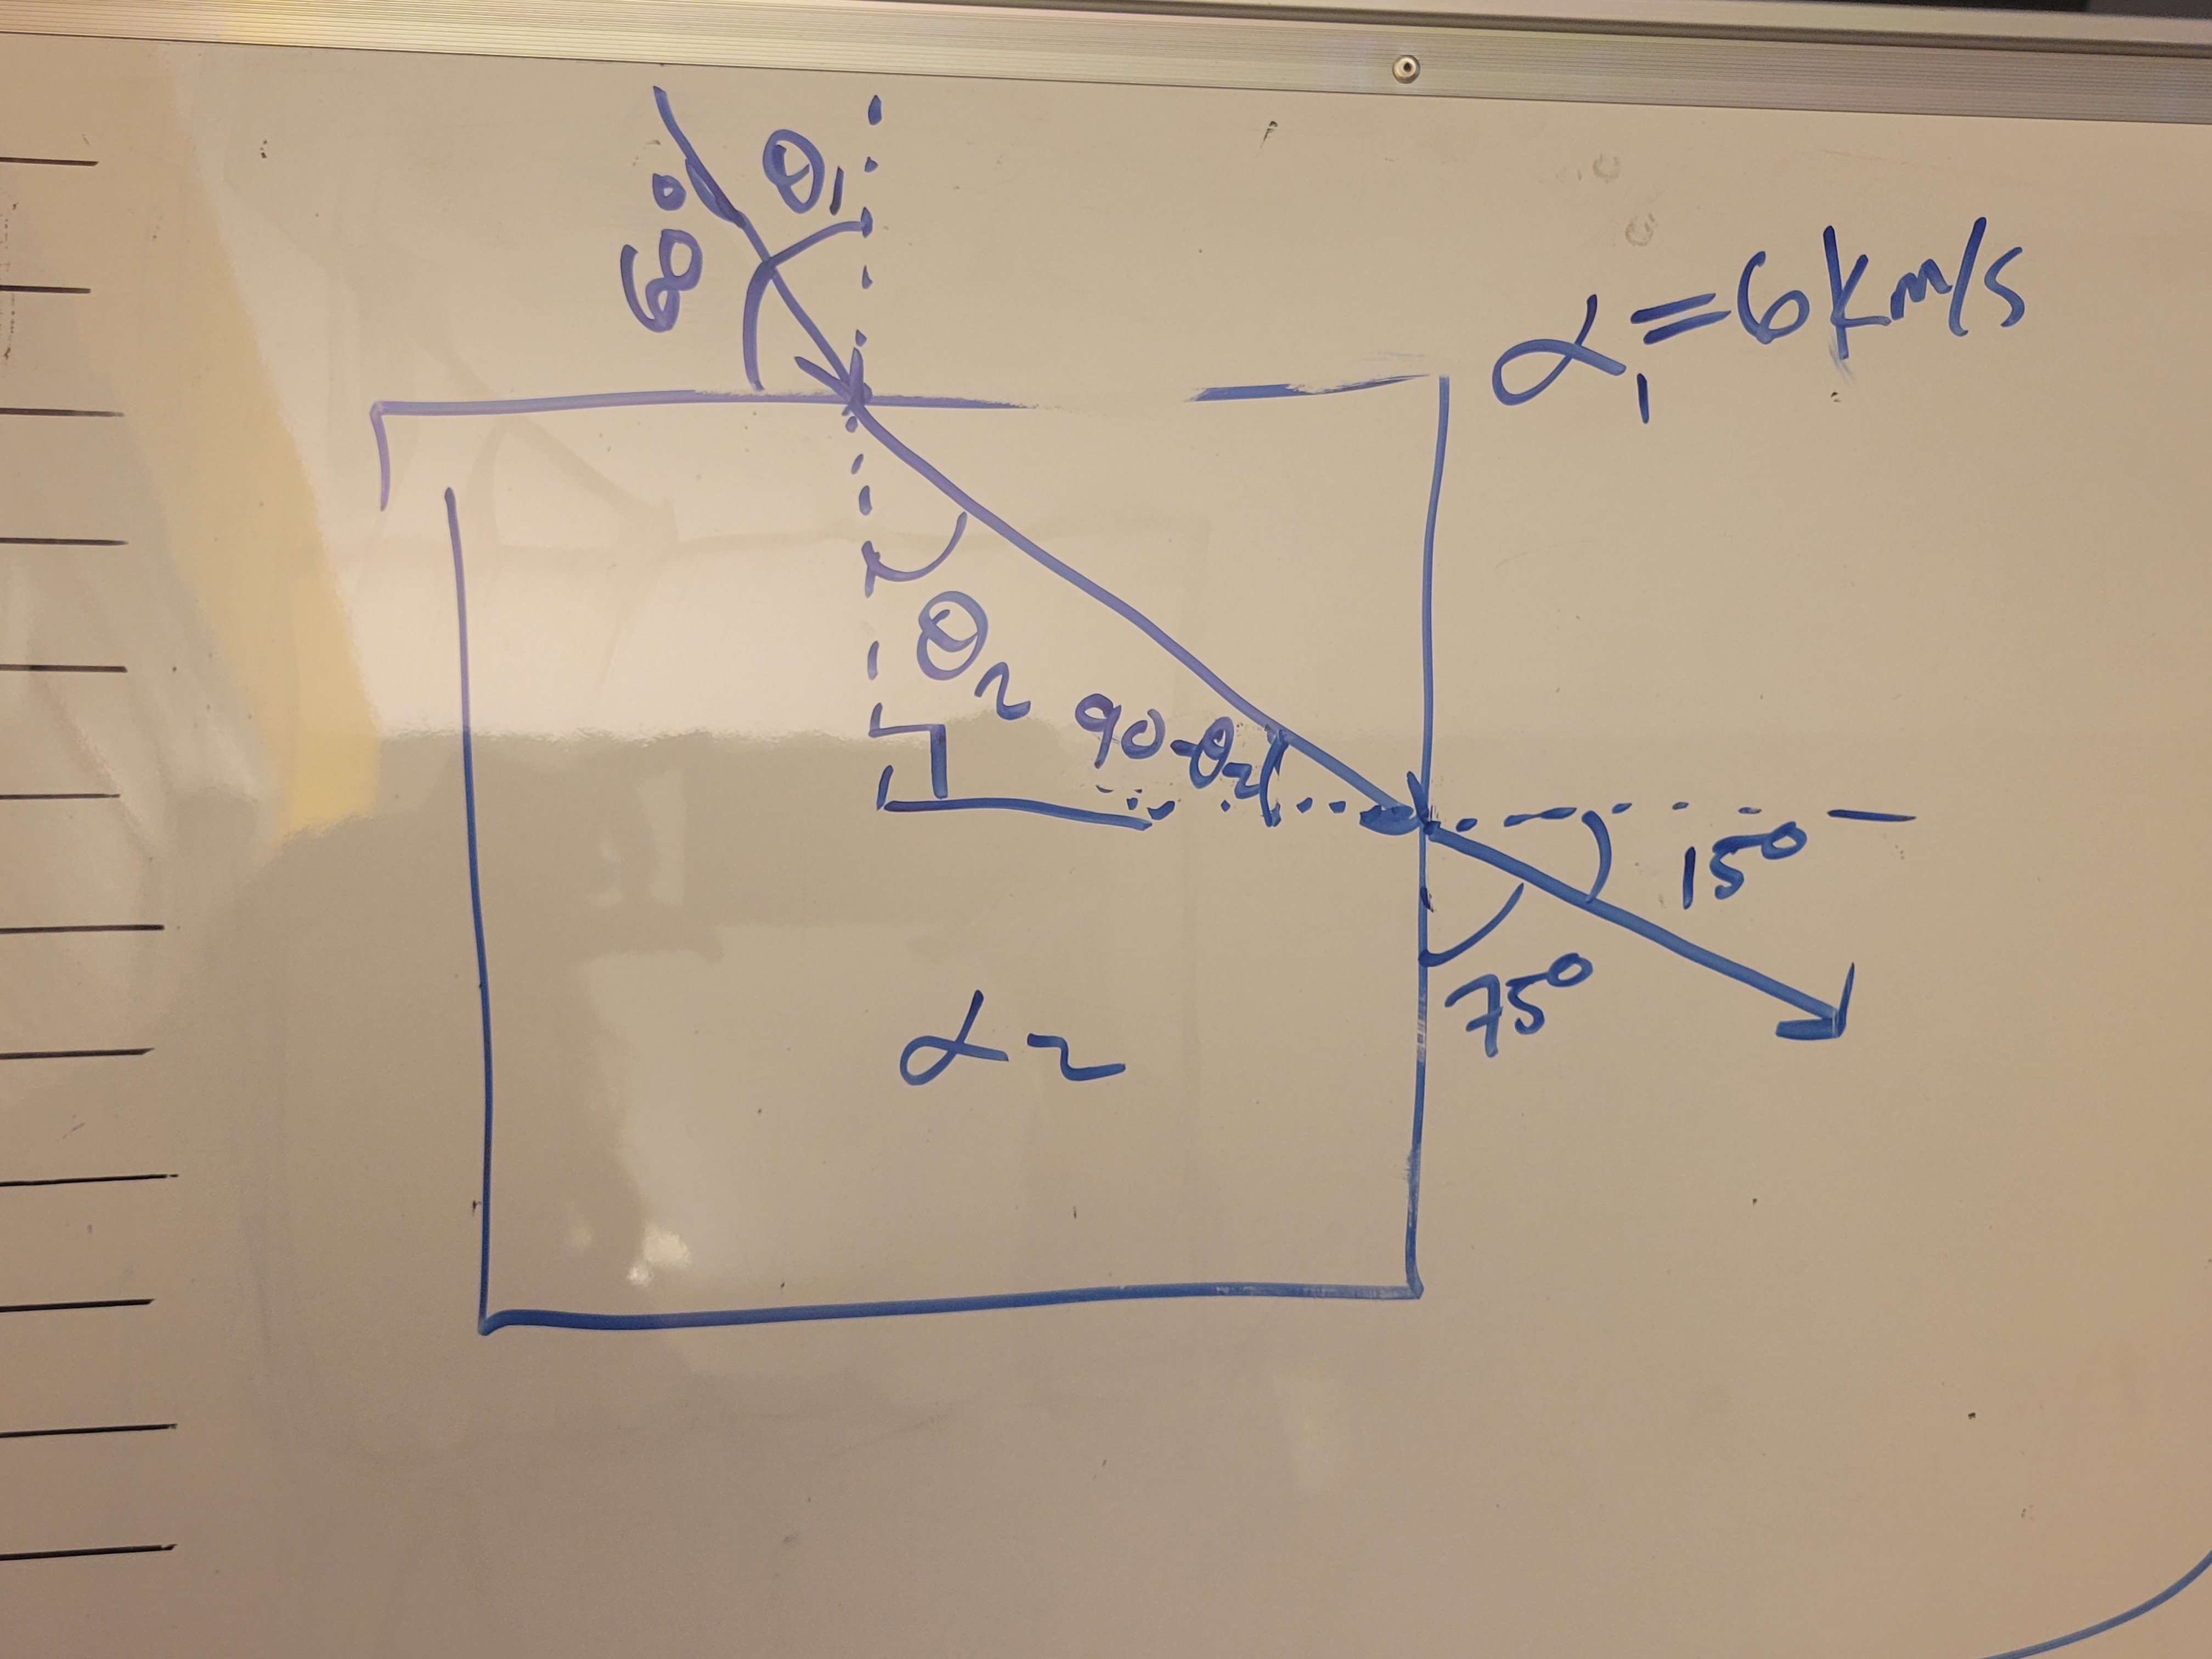
\includegraphics[width=0.5\textwidth]{box_alpha.jpg}
\end{figure}

A downgoing P wave in a medium with a P velocity of 6 km/s travels through this “corner” shaped structure. If the incident ray is at an angle of $60^\circ$ from the horizontal and the final ray is at an angle of $75^\circ$ from the vertical, what is the P velocity within the corner-shaped medium?\\

Start with Snell's Law to find $\alpha_{2}$ and write two equations for the two unkowns.\\

\begin{center}
$\frac{\sin{\theta{1}}}{\alpha_{1}} = \frac{\sin{\theta_{2}}}{\alpha_{2}}$ and $\frac{\left(\sin90 - \theta_{2}\right)}{\alpha_{2}} = \frac{\sin{\theta_{3}}}{\alpha{1}}$ where $\theta_{1} = 30^\circ$ and $\theta_{3} = 15^\circ$ and $\alpha_{1} = 6$.
\end{center}

$\alpha_{2} = \frac{\alpha_{1}\sin\left(90 - \theta_{2}\right)}{\sin{\theta_{3}}} = \frac{\alpha_{1}\cos\theta_{2}}{\sin{\theta_{3}}}$ and $\alpha_{2} = \frac{\alpha_{1}\sin\theta_{2}}{\sin{\theta_{1}}} \rightarrow \frac{\cancel{\alpha_{1}}\cos\theta_{2}}{\sin{\theta_{3}}} = \frac{\cancel{\alpha_{1}}\sin\theta_{2}}{\sin{\theta_{1}}} \Rightarrow \frac{\sin{\theta_{1}}}{\sin{\theta_{3}}} = \tan{\theta_{2}} \Rightarrow \theta_{2} = \tan^{-1}{\frac{\sin{\theta_{1}}}{\sin{\theta_{3}}}}$  

$\alpha_{2} = \alpha_{1} \frac{
\cos\left(\theta_{2}
	\right)}
{\sin{\theta_{3}}} = 10.66 \frac{km}{s}$




\section{}
We can re-write $\mu$ in terms of $\beta$ and $\rho$ as $\mu = \beta^{2} \rho$. Now:

\[
h\omega\sqrt{\frac{1}{\beta_{1}^{2}} - \frac{1}{c^{2}}} = \tan^{-1}\left[
	\frac{\beta_{2}^{2}\rho_{2}\sqrt{\frac{1}{c^{2}} - \frac{1}{\beta_{2}^{2}}}}{\beta_{1}^{2}\rho_{1}\sqrt{\frac{1}{\beta_{1}^{2}} - \frac{1}{c^{2}}}}
\right] \Rightarrow \omega = \frac{\tan^{-1}\left[
	\frac{\beta_{2}^{2}\rho_{2}\sqrt{\frac{1}{c^{2}} - \frac{1}{\beta_{2}^{2}}}}{\beta_{1}^{2}\rho_{1}\sqrt{\frac{1}{\beta_{1}^{2}} - \frac{1}{c^{2}}}}
\right]}{h\sqrt{\frac{1}{\beta_{1}^{2}} - \frac{1}{c^{2}}}}
\]


\end{document}
